%!TEX root = ../../dokumentation.tex
\textbf{Synchronous Messaging}

For synchronous messaging, the architectural concept of \ac{REST}, the \ac{RPC} framework \textit{gRPC} and lastly the data query language and runtime \textit{GraphQL} are presented.
Although a lot more alternatives are available, the aforementioned options each represent vastly different concepts.
They are selected as they are the most recent and widespread used technology in their category \cite{Mohilo.2019}\cite{Smith.382018}.
Alternatives to \ac{REST} could be \textit{SOAP} (over \ac{HTTP}) for instance.
Likewise, instead of \textit{gRPC}, implementations such as Java RMI, Apache Thrift or even XML-RPC (precursor to \textit{SOAP}) would be viable options as well \cite{Giro.2019}\cite[p.~62f.]{Bruce.2019}.

\subsection{RESTful HTTP}\label{cha:Technologies:communication:rest}

\acf{REST} is an architectural style which focuses on the concept of resources.
Resources shown externally can be completely decoupled from its internal format.
Furthermore, the resources can be encoded in any arbitrary format, such as \ac{HTML}, \ac{XML} or \ac{JSON} and are accessed through resource methods \cite{Restfulapi.net.23.05.2020}.
A further description of the total 6 guiding principles can be seen in Fieldings work \cite{Fielding.15.03.2002}.
In theory \ac{REST} can be used with any underlying protocol, however, in practice \ac{REST} is commonly used together with \ac{HTTP}, hence the name RESTful \ac{HTTP}.
A widely used and recommended model is the Richardson Maturity Model, which describes resource management, the usage of \ac{HTTP} verbs and hypermedia controls \cite{Fowler.2010}.

With the use of \ac{HTTP}, verbs such as \textit{GET}, \textit{POST}, \textit{DELETE}, single endpoints serving multiple purposes are possible, as seen in Table \ref{tab:restExample}.
Furthermore, support of RESTful communication for proxies, caching services and load balancers as well as security measures is available due to the \ac{HTTP} ecosystem.
On the one hand this fact can make \ac{REST} easy to adopt and to ensure interoperability with preexisting architectures.
On the other hand however, this also leads to the necessity of a secure and scalable communication infrastructure (e.g. use of \ac{TLS} for encryption ) as a base \cite[p.~100]{Newman.2015}.

Another benefit, that RESTful communication provides (if implemented according to the Richardson Maturity Model), is the hypermedia control for resources or \enquote{Hypermedia as the enginge of application state} (HATEOAS).
The concept of hypermedia allows clients to perform interactions with the referenced links, embedded in the response.
As requests are only bound to a reference and not beforehand known direct endpoints, clients are abstracted and the implementation can be changed, as long as the semantic of a response does not change.
Consequently, both client and server implementations are decoupled, as the common denominator is the hypermedia control.
Due to the progressive discovery of the \ac{API} that this hypermedia approach entails, the communication may be more verbose, compared to other technologies.

\begin{table}
	\centering
	\begin{tabular}{ |l|l| }
		\hline
		Action               & REST operation               \\
		\hline
		Get news item        & /news/\{id\} \textbf{GET}    \\
		Get (all) news items & /news/ \textbf{GET}          \\
		Delete news item     & /news/\{id\} \textbf{DELETE} \\
		Update news item     & /news/\{id\} \textbf{PUT}    \\
		Create news item     & /news/\{id\} \textbf{POST}   \\
		\hline
	\end{tabular}
	\caption{Exemplary \ac{REST} operations on news item object} \label{tab:restExample}
\end{table}

\subsection{ gRPC}\label{cha:Technologies:communication:grpc}

Developed in 2015 by Google, \textit{gRPC} is an open source \ac{RPC} system, which uses HTTP2 for transport \cite{gRPCAuthors.25.05.2020}.
As it is an \ac{RPC} framework, characteristics, such as tighter coupling, but on the other hand also high performance messaging apply \cite[p.~93f.]{Newman.2015}.
Likewise server and client code can be generated automatically for a variety of targets.
In the case of \textit{gRPC}, as of May 2020, 11 languages are officially supported, namely \textit{C/C++, C\#, Dart, Go, Java, Kotlin, Node.js, Objective-C, PHP, Python, Ruby}.

Unlike \ac{REST}, \textit{gRPC} relies on an \ac{IDL} to define the services, which per default are \textit{protocol buffers} (often abbreviated as \enquote{protobuf})
Apart from using protocol buffers as its \ac{IDL}, \textit{gRPC} can also use it as its message interchange format.
In order for \textit{gRPC} to be able to serialize structured data, each data type may be described in a \textit{*.proto} file, although other similar and popular \acp{IDL}, such as Apache Thrift, as well as \ac{JSON} or \ac{XML} are supported \cite{gRPCAuthors.25.05.2020b}\cite{gRPCAuthors.25.05.2020d}. \\

\begin{lstlisting}[caption=Example of data structure in a \textit{*.proto} file, label=listing:protobufdata]
message Studienarbeit {
string title = 1;
int32 id = 2;
bool passed = 3;
}
\end{lstlisting}

\begin{lstlisting}[caption=Example of service definition in a \textit{*.proto} file, label=listing:protobufservice]
service Greeter {
// Sends a greeting
rpc SayHello (HelloRequest) returns (HelloReply) {}
}

// The request message containing the user's name.
message HelloRequest {
string name = 1;
}

// The response message containing the greetings
message HelloReply {
string message = 1;
}
\end{lstlisting}

An example of such a data object description, using a protocol buffer definition can be seen in Listing \ref{listing:protobufdata}.
With a proto file, according stubs can be generated for target programming languages, by using the protocol buffer compiler \textit{protoc}.
Services to be used can be defined in \textit{gRPC} as well, as seen in Listing \ref{listing:protobufservice} \cite{gRPCAuthors.25.05.2020b}\cite{gRPCAuthors.25.05.2020c}.
The code generated by \textit{protoc} in according target languages can then be used in server and clients as depicted in Figure \ref{img:grpcoverview} \cite{gRPCAuthors.25.05.2020b}.

\begin{figure}[hb]
	\centering
	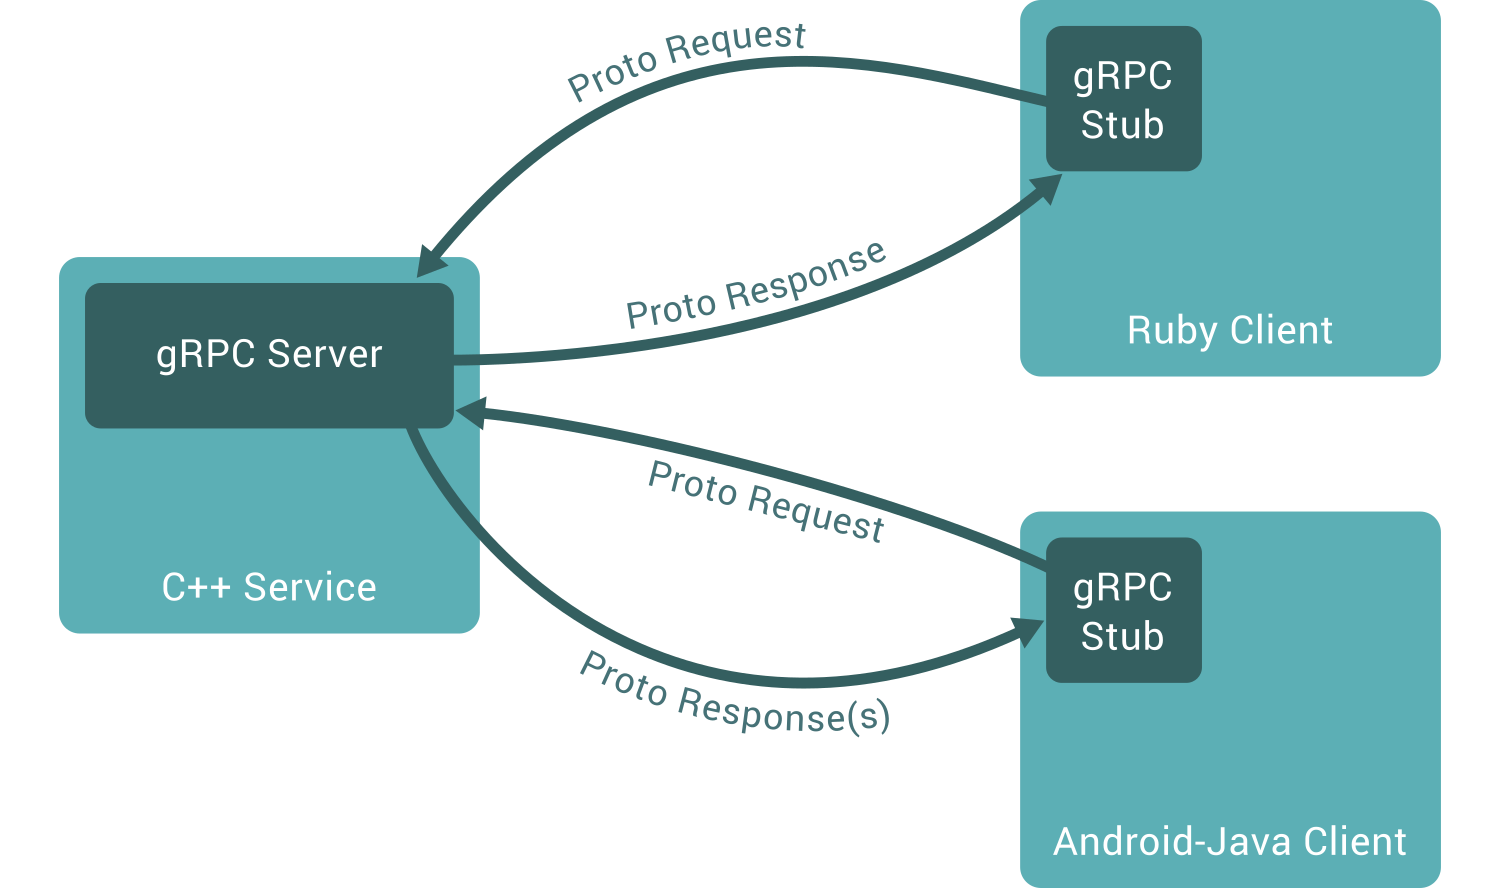
\includegraphics[width=\textwidth, height=0.25\textheight, keepaspectratio]{gRPCoverview.png}
	\caption{gRPC polyglot implementation overview}
	\label{img:grpcoverview}
\end{figure}

A common use case for \textit{gRPC} currently is the inter service communication in microservices, especially, where strict specification and low latency actions need to be executed \cite{Sturgeon.2016}.
The concept of \textit{gRPC} is based around an API contract and strict semantics.
Protocol buffer as a small binary format has a faster serialization (\enquote{de-/marshalling}) and is more efficient, in contrast to the human readable \ac{JSON} used in RESTful \ac{HTTP} applications.
This makes \textit{gRPC} especially useful for network constrained environments and high throughput communication.
As protocol buffer serves as an \ac{IDL}, \textit{gRPC} user have to follow a prescriptive formal specification, as opposed to loose models and implementation levels (e.g. Richardson Maturity Model) \cite{NewtonKing.2019}.

Furthermore, due to the use of HTTP2, \textit{gRPC} supports bi directional streaming, making point-to-point real time communication possible.
Consequently, the need for polling or switching protocols to \textit{WebSocket} for instance can be eliminated.
Other supported forms of streaming are server to client, client to server and unary.

In contrast to \ac{REST}, the usage of \textit{gRPC} in the browser is limited and not supported by default.
Consequently extensions like \textit{gRPC-Web} are needed, which includes an \textit{gRPC} proxy and a JavaScript client for the browser.
Furthermore, \textit{gRPC} messages can not be broadcasted and are not human readable due to protocol buffers being a binary format.
Nonetheless \textit{gRPC} represents a well supported \ac{RPC} communication framework, which is beneficial for efficient inter process communication in distributed client server architectures.
Especially in the context of polyglot microservice environments, the streaming capabilities and low latency of \textit{gRPC} are useful, not only for backend communication but also for applications on (mobile) clients \cite{NewtonKing.2019}\cite{1&1IONOSSE.2020}.

\subsection{GraphQL}\label{cha:Technologies:communication:graphql}

\textit{GraphQL} can be defined as both a data query language as well as a runtime.
The language is used for writing requests for client applications and is close to
\ac{JSON} (as seen in Listing \ref{listing:graphqlquery}).
Contrary to that, the \textit{GraphQL} runtime layer is needed on the server, in order to transform requests into existing logic to fetch data \cite[p.7~f.]{Buna.2016}.
The runtime layer is also responsible for accumulation of different data sources (e.g. composite design pattern seen in Figure \ref{img:compositedesigngraphql})
Although the service is transport agnostic, the most common combination is with \ac{HTTP}.
Furthermore, \textit{GraphQL} has a widespread implementation available similar to \textit{gRPC}, namely \textit{C\# / .NET, Clojure, Elixir, Erlang, Go, Groovy, Java, JavaScript, Julia, Kotlin, Perl, PHP, Python, R, Ruby, Rust, Scala, Swift, OCaml / Reason} \cite{TheGraphQLFoundation.27.05.2020}.

\begin{figure}
	\centering
	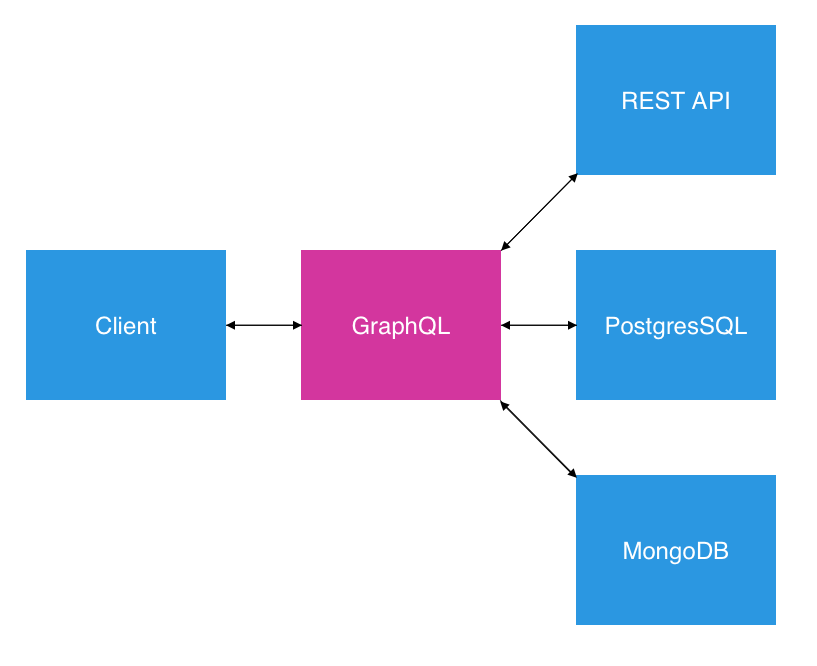
\includegraphics[width=\textwidth, height=0.32\textheight, keepaspectratio]{compositedesigngraphql.png}
	\caption{Composite design pattern in \textit{GraphQL} \cite{Lombard.2018}}
	\label{img:compositedesigngraphql}
\end{figure}

With \textit{GraphQL}, the client specifies the data requirements and only requests the data they need, hence often being referred to as an declarative data fetching language \cite[p.~6f.]{Buna.2016}.
In Listing \ref{listing:graphqlquery} two queries are described, with the according responses seen in Listing \ref{listing:graphqlresponse}.
With the second query, the main characteristics of \textit{GraphQL} are visible \cite[p.~16]{Porcello.2018}:

The data that is served is strongly typed in the \textit{GraphQL} scheme, which makes misuse detection easier \cite[p.~65]{Buna.2016}.
Each data point has a specific type, the scheme \textit{person} has to exist, with predefined field types, such as \textit{filmConnection} as a \textit{PersonFilmsConnection}.
Furthermore \textit{GraphQL} is product centric, which means that it is focused on the clients data needs and the supporting language and runtime.
This also allows for client-specified queries; servers have to provide the capabilities that clients are allowed to consume.
The field \textit{filmConnection} as well as the schemes for the object \textit{films} therefore have to exist.

In cases where the client does not know about the server's type system, the client has to be able to query the scheme with the \textit{GraphQL} language (\textit{Introspection}).
Lastly, every \textit{GraphQL} query can be hierarchical.
Fields can be nested in other fields, as seen with \textit{films} via the \textit{filmConnection}, and the corresponding response is shaped exactly the same \cite[p.~12ff.]{Porcello.2018}\cite[p.~10ff.]{Buna.2016}.

\begin{lstlisting}[caption=Example of GraphQL queries, label=listing:graphqlquery]
// first query
query{
person(personID>5) {
name,
birthYear
}
}
// second query with more fields
query{
person(personID>5) {
name,
birthYear,
filmConnection {
films {
title
}}}
}
\end{lstlisting}

\begin{lstlisting}[caption=Example of GraphQL responses, label=listing:graphqlresponse]
// response to the first query
{
"data": {
"person": {
"name": "Leia Organa",
"birthYear": "19BBY",
}}
}

// response to the second query
{
"data": {
"person": {
"name": "Leia Organa",
"birthYear": "19BBY",
"filmConnection": {
"films": [
{"title":"A New Hope"},
{"title":"The Empire Strikes Back"},
{"title":"The Force Awakens"},
]
}}}
}
\end{lstlisting}

Further exact description about the query language and the scheme as well as the configuration of the runtime are left out in this work, as they are not required for an overview here.

\textit{GraphQL} currently is mostly recommended for Data \acp{API}, especially when the requested data is graph-like.
Similar to \textit{gRPC}, the efficiency through direct querying and low latency, due to the most minimal response size, make \textit{GraphQL} especially useful for applications with a restricted bandwith (e.g. mobile appliances).
RESTful \ac{API} in contrast, may suffer from over- and/or underfetching \cite[p.~3]{Doerrfeld.2018}.

Overfetching occurs when more data is given than actually needed, which may happen especially with large data endpoints with HATEOAS implemented.
On the other hand, when needed data is undercut, the client would have to make multiple requests.
Especially on resource restricted devices, multiple round trips for a single view are inefficient \cite[p.~12f.]{Buna.2016}\cite[p.~24ff.]{Porcello.2018}.
This issue is mitigated in \textit{GraphQL}, as the response is uniform with the request itself.
Moreover, nesting reduces the load on the target device.
In a RESTful API, in order to receive the data of the second request depicted in Listing \ref{listing:graphqlquery}, one would request the \textit{films} of a \textit{person} and receive \textit{filmCollection}, a list of links.
Following that, each link would have to be requested and the field \textit{title} extracted.

\begin{figure}[h]
	\centering
	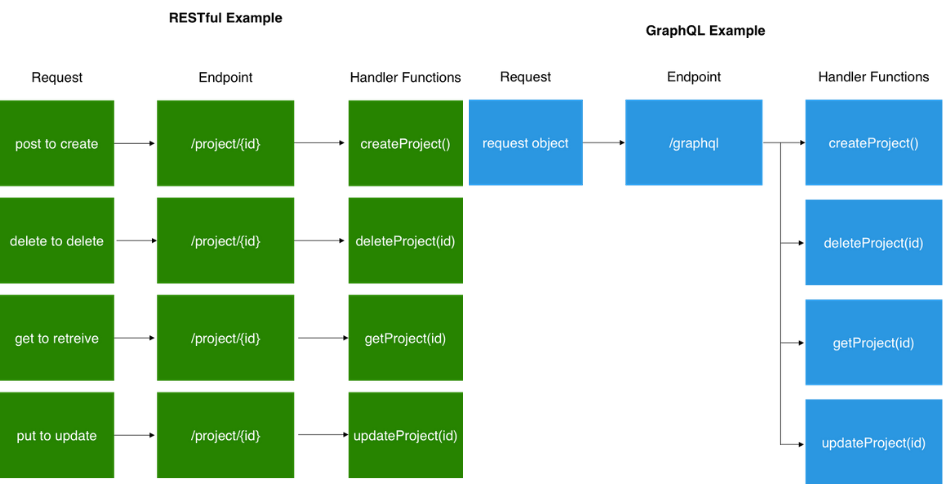
\includegraphics[width=\textwidth, height=0.9\textheight, keepaspectratio]{multiplerestVSgraphql.png}
	\caption{Multiple REST requests vs a single GraphQL request \cite{Lombard.2018}}
	\label{img:restvsgraphqlrequest}
\end{figure}

Furthermore \textit{GraphQL} is easier to scale and maintain due to stronger typing and schema discovery.
Although RESTful \ac{API} implements this with HATEOAS, versioning of endpoints or managing endpoints in general can be cumbersome.
With \textit{gRPC}, flexibility is very limited as it is an \ac{RPC} framework in its nature.
\textit{GraphQL} instead resolves this, by having only one endpoint, with which balancing, orchestration of data sources and version control is possible. (cf. Figure \ref{img:restvsgraphqlrequest})
Consequently, \textit{GraphQL} is the most flexible and scalable when comparing against \textit{gRPC} or a RESTful \ac{HTTP} \ac{API} \cite[p.~29]{Porcello.2018}\cite[p.~11]{Buna.2016}.

Nonetheless, \textit{GraphQL} can be at a disadvantage due to incompatibility with common caching solutions and query complexity.
Each query still needs to be resolved with the target data source, where bottlenecks naturally occur.
This issue especially prevails in situations with a high query depth or query complexity.
Furthermore, rate limiting as typically applied in RESTful \acp{API} are more difficult to apply, because the query depth and complexity weighing can vary a lot \cite{Wieruch.2018}\cite{AltexSoft.2019}.
In most cases, however, \textit{GraphQL} is used as an intermediary, where a \textit{GraphQL} \ac{API} is exposed, but the runtime itself communicates over existing \ac{REST} \acp{API}.
This hybrid proxy variant allows easy adoption and a incremental adoption of \textit{GraphQL} \cite[p.~29]{Porcello.2018}.
